\section{Problem Description}
\label{c:prob_desc}
% 先描述Motivations和Motivating examples. 

% Problem definition

In order to avoid struggling with low-level details when programming IoT applications, we need to hide the low-level details which means we have to increase the level of programming abstraction in IoT systems. 

Everything has an identifier so that is manageable and inventoried by computers in IoT's vision, so that everything can be seen as a service\cite{Perera2014}. Every objects with sensing, actuating, computing capabilities can be abstracted to an IoT service. The definition of an IoT service in our system is shown as following, 

\begin{defn}
An IoT service can be represented as $S = \lbrace N, S, L, In, Out, Q \rbrace $,
\end{defn}

% 解釋Definition
% 簡單敘述下Service定義下所有IoT service怎麼樣子被表示
where $N$ represents for the service identification. $S$ and $L$ represents the low-level details of this service, where $S$ is the service set contained by this service, and $L$ is the relationship of services in $S$. $In$ and $Out$ are the input/output ports that the service exposes. $Q$ is the set of attributes for this service. Primitive sensing such as illuminance, temperature, humidity can be categorized as atomic services. Composite sensing such as foot step sensor, pollution index sensor can also be expressed by our service definition. For more complicted service, an IoT application can be expressed by this definition as figure \ref{fig_service_example} shows.

\begin{figure}[!t]
\centering
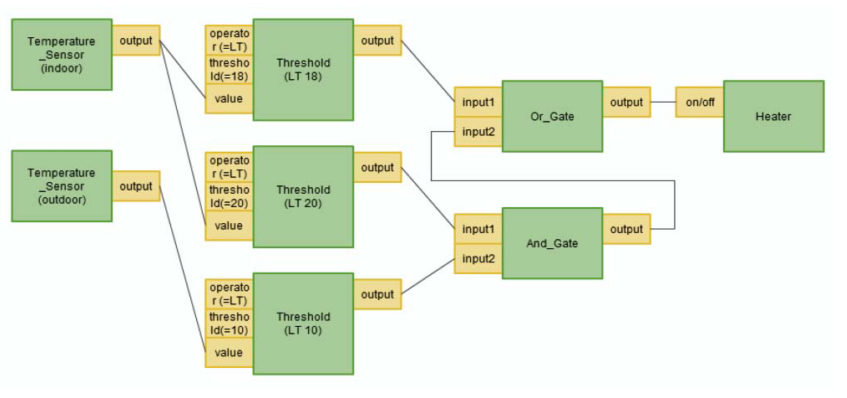
\includegraphics[width=1.0\columnwidth]{service_example}
\caption{Example service abstraction and composition in WuKong system.}
\label{fig_service_example}
\end{figure}

% 一隻program要可以deploy到很多地方

Programming on IoT system is not simple. WuKong was proposed to support service-oriented programming paradigm\cite{Lin2013}. We used flow-based programming as a tool for user to express their requirements as an abstraction of data flow. Then WuKong master would compile and map the virtual application into physical device.  Although lots middleware solutions including WuKong have been proposed to support programming IoT as a system instead of node by node, programming IoT still requires certain low-level understanding on target environment. Programmer in WuKong would have to modify program whenever the target environment changes, or user requirements change, which is considered not an elegant and efficient way. 

% 有很多類型的low-level details會增加programmer的complexity
% Sensing/Actuating Coverage, QoI, QoS, Compound service
There are many kinds of low-level details that will increase the complexity during the development of IoT application. For sensor deployment in wide area, we might deploy more than one sensors for sensing coverage. For actuating coverage, we might like to control the brightness in conference room as a whole instead of every single light. Redundancy helps to resolve sensor failures and sensor anomalies. For a better quality of information(QoI), we can set redundant sensors to ensure a more stable sensor reading value. Redundant sensors or actuators can also improve the reliability and availability which are quality of service(QoS). High-level contextual data will have different solutions to achieve by utilizing primitive sensor reading value. For example, there could exists at least two solutions for foot step sensor, one is to utilize a sound sensor and a fast-fourier transformation component, while another one is to utilize a pressure sensor on the ground. 


%For example, light sensor can be seen as a service, light actuator can also be seen as a service, threshold computing object can be seen as a service [左圖] also. 
% 簡單敘述從原本的1對1 mapping, 我想把QoS support加入去挑最好的1-to-1 mapping, 進一步的不只有1-to-1 mapping還有1-to-many mapping, many-to-1 mapping.
With the goal to hide low-level details of a service, middleware solution should support programmer to match their application to a set of desired physical resources by considering user QoS requirements. Furthermore, every service components in an application should not be restricted to one-to-one mapping between abstract services and physical resources. Many-to-one and one-to-many mapping are very important for achieving the goal of hiding low-level details for programmers.
